\documentclass[conference]{IEEEtran}
\IEEEoverridecommandlockouts
% The preceding line is only needed to identify funding in the first footnote. If that is unneeded, please comment it out.
\usepackage{cite}
\usepackage{amsmath,amssymb,amsfonts}
\usepackage{algorithmic}
\usepackage{graphicx}
\usepackage{textcomp}
\usepackage{xcolor}
\usepackage[brazilian]{babel}
\usepackage[utf8]{inputenc}
\usepackage[T1]{fontenc}
\def\BibTeX{{\rm B\kern-.05em{\sc i\kern-.025em b}\kern-.08em
    T\kern-.1667em\lower.7ex\hbox{E}\kern-.125emX}}
\begin{document}

\title{Particle Swarm Optimization}

\author{Bruno Lopes}
\maketitle

\begin{abstract}
O objectivo deste artigo é conseguir implementar e avaliar a eficiência de Algoritmos de Otimização por Enxame de Partículas.

\end{abstract}

\section{INTRODUÇÃO}
	A otimização de enxame de partículas (PSO) é uma das técnicas evolutivas de computação. Como as outras técnicas de computação evolutiva, o PSO é um algoritmo de busca baseado na população e é inicializado com uma população de soluções aleatórias, chamadas partículas. Ao contrário das outras técnicas de computação evolucionária, cada partícula em PSO também está associada a uma velocidade. Partículas voam através do espaço de busca com velocidades que são ajustadas dinamicamente de acordo com seus comportamentos históricos. Portanto, as partículas tendem a voar em direção à melhor e melhor área de pesquisa ao longo do processo de busca. Desde sua introdução em 1995 \cite{b1}, a PSO atraiu muitas atenções de pesquisadores de todo o mundo. Muitos resultados de pesquisa foram relatados na literatura. Em 2003, o primeiro Simpósio IEEE sobre Inteligência de Enxame foi realizado em Indianápolis, Indiana, EUA. 
		
	As pesquisas sobre PSO geralmente podem ser categorizadas em cinco partes: algoritmos, topologia, parâmetros, algoritmos de PSO híbridos e aplicativos.

\section{Referencial Teórico}

Algoritmos Genéticos são algoritmos de otimização global, baseados nos mecanismos de seleção natural e da genética \cite{b2}. Eles empregam uma estratégia de busca paralela e estruturada, mas aleatória, que é voltada em direção ao reforço da busca de pontos de "alta aptidão", ou seja, pontos nos quais a função a ser minimizada (ou maximizada) tem valores relativamente baixos (ou altos).

Os princípios da natureza nos quais os GAs se inspiram são simples. De  acordo com  a teoria de C. Darwin, o princípio de seleção privilegia os indivíduos mais aptos com maior longevidade e, portanto, com maior probabilidade de reprodução. Indivíduos  com  mais descendentes têm mais chance de perpetuarem seus códigos genéticos nas próximas   gerações.

Os algoritmos genéticos foram introduzidos por J. Holland em 1975 \cite{b1} com o objetivo de formalizar matematicamente e explicar rigorosamente processos de adaptação em sistemas naturais e desenvolver sistemas artificiais artificiais (simulados em computador) que retenham os mecanismos originais encontrados em  sistemas  naturais. 

Em 1975, Holland publicou o livro Adaptation in Natural and Artificial Systems, hoje considerado a Bíblia de Algoritmos Genéticos. Desde então, estes algoritmos vêm sendo aplicados com sucesso nos mais diversos problemas de otimização e aprendizado de máquina. 

Os AG's possuem uma larga aplicação em muitas áreas científicas, entre as quais podem ser destacadas:
    
    \begin{itemize}
    \item Síntese de circuitos analógicos:  para uma certa entrada e uma saída desejada, por exemplo tensão, o AG gera a topologia , o tipo e o valor dos componentes do circuito.

    \item Síntese de protocolos:  determinação de quais funções do protocolo devem ser implementadas em hardware e quais devem ser implementadas em software para que um certo desempenho seja alcançado.

    \item Programação Genética: gera a listagem de um programa, numa determinada linguagem especificada, para que um determinado conjunto de dados de entrada forneça uma saída desejada.

    \item Gerenciamento de redes: supervisão do tráfego nos links e das filas nos "buffers" de roteadores para descobrir rotas ótimas e para reconfigurar as rotas existentes no caso de falha de algum link.

    \item Computação Evolutiva: gera programas que se adaptam a mudanças no sistema ao longo do tempo.

    \item Otimização evolutiva multi-critério: otimização de funções com múltiplos objetivos que sejam conflitantes.

    \item Problemas de otimização complexos: problemas com muitas variáveis e espaços de soluções de dimensões elevadas. Ex: problema do caixeiro viajante, gerenciamento de carteiras de fundos de investimento.

    \item Ciências biológicas:  modela processos biológicos para o entendimento do comportamento de estruturas genéticas.

    \item Autômatos auto-programáveis.
    \end{itemize}

A idéia básica de funcionamento dos algoritmos genéticos é a de tratar as possíveis soluções do problema como "indivíduos" de uma "população", que irá "evoluir" a cada iteração ou "geração". Para isso é necessário construir um modelo de evolução onde os indivíduos sejam soluções de um problema. 

 A estrutura geral do programa está apresentada na Figura1 e os detalhes da execução do algoritmo pode ser resumida nos seguintes passos:
    \begin{itemize}
    \item População inicial, normalmente formada por indivíduos criados aleatoriamente;
    Avaliar a população de indivíduos segundo algum critério de qualidade (função de aptidão ou "fitness");
    
    \item Em seguida, através do operador de "seleção", escolhem-se os indivíduos de mais aptos com maior longevidade para a criação de um novo conjunto de possíveis soluções, chamado de nova "geração";
    
    \item Esta nova geração é obtida aplicando-se sobre os indivíduos selecionados operações que misturem suas características (chamadas "genes"), através dos operadores de "cruzamento" ("crossover") e "mutação";
    
    \item Estes passos são repetidos até que uma solução aceitável seja encontrada, até que o número predeterminado de passos seja atingido ou até que o algoritmo não consiga mais melhorar a solução já encontrada.
    \end{itemize}
    
    \begin{figure}[htbp]
    \centerline{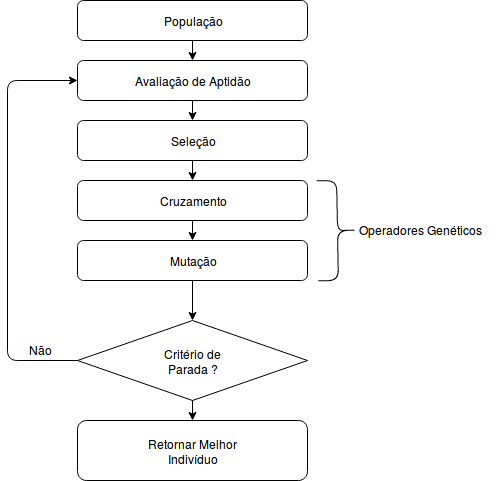
\includegraphics[scale=0.4]{algoritmo-genetico.png}}
    \caption{Estrutura básica de um algoritmo}
    \label{fig}
    \end{figure}
    
    Até o presente momento todos os fundamentos apresentados basearam-se na nos algoritmos genéticos simples. Existem outros tipos de algoritmos genéticos que foram desenvolvidos para problemas mais específicos.
    
\section{Metodologia Experimental}

Em geral, um AG possui duas categorias de parâmetros da pesquisa experimental: qualitativos e quantitativos. Os principais parâmetros qualitativos são os tipos de crossover (um ponto, dois pontos e múltiplos pontos) e os métodos de seleção (proporcional, escalonamento, Boltzmann, ranqueamento e tournament). Os principais parâmetros quantitativos são constituídos pelo tamanho da população (n), pela taxa de crossover (TC) e pela taxa de mutação (Tm). 

Para os experimentos realizados neste trabalho, utilizamos somente a metodologia quantitativa pois somente os parâmetros básicos foram alterados. Como por exemplo: tamanho da população, taxa de crossover e mutação além do tamanho do genótipo a ser encontrado.

Os objectivos da investigação quantitativa consistem essencialmente em encontrar relações entre variáveis, fazer descrições recorrendo ao tratamento estatístico dos dados recolhidos, testar teorias e tirar conclusões.

\section{Resultado e Discussão}

Na Tabela 1 estão resumidos os resultados dos experimentos realizados. Pode-se observar que as mudanças realizadas na taxa de crossover e mutação influenciam de forma significativa no número de iterações necessárias para encontrar o genótipo.  

Mas se esta for muito alta, estruturas com boas aptidões poderão ser retiradas mais rápida um valor alto, a maior parte da população será substituída, mas com valores muito altos pode ocorrer perda de estruturas de alta aptidão. Com um valor baixo, o algoritmo demorou um tempo maior para convergir.

    \begin {table}
    \caption {Resumo experimentos}
    \begin{center}
      \begin{tabular}{ l | c | r }
        \hline

        20&	16&	10.00 \\
        \hline
      \end{tabular}
      \end{center}
    \end{table}

Uma baixa taxa de mutação previne que uma dada posição fique estagnada em um valor, além de possibilitar que se chegue em qualquer ponto do espaço de busca. Com uma taxa muito alta a busca se torna essencialmente aleatória.
    
Vale ressaltar que o algoritmo de seleção utilizado nos experimentos foi o seleção por roleta. Quanto melhores são os cromossomos, mais chances de serem selecionados, mas por outro lado, existe a probabilidade da perda do melhor indivíduo.

\section*{Conclusão}

O principal objetivo deste trabalho foi entender o funcionamento de um algoritmo genético clássico e desenvolver uma solução que pudesse gerar novos indivíduos, até que um determinado genótipo fosse encontrado. Foram testados os efeitos dos parâmetros passados para o método de crossover, tamanho da população e taxa de mutação. Foi possível perceber que houve diferenças na quantidade de gerações necessárias para encontrar o genótipo, levando em consideração a quantidade de indivíduos, taxa de crossover e mutação.

O melhor desempenho do algoritmo genético é dependente da escolha de uma boa configuração de seus parâmetros.


\begin{thebibliography}{00}

\bibitem{b1} Kennedy, J., and Eberhart, R. C.. (1995). Particle swarm optimization, Proc. of IEEE International Conference on Neural Networks (ICNN), Vol.IV, pp.1942-1948, Perth, Australia, 1995.
\end{thebibliography}
\vspace{12pt}

\end{document}
